\documentclass[12pt,letterpaper]{exam}
\usepackage[lmargin=1in,rmargin=1in,tmargin=1in,bmargin=1in]{geometry}
\usepackage{../style/exams}

% -------------------
% Course & Exam Information
% -------------------
\newcommand{\course}{MAT 101: Exam 2}
\newcommand{\term}{Winter -- 2021}
\newcommand{\examdate}{01/14/2021}
\newcommand{\timelimit}{95 Minutes}

\setbool{hideans}{false} % Student: True; Instructor: False

% -------------------
% Content
% -------------------
\begin{document}

\examtitle
\instructions{Write your name on the appropriate line on the exam cover sheet. This exam contains \numpages\ pages (including this cover page) and \numquestions\ questions. Check that you have every page of the exam. Answer the questions in the spaces provided on the question sheets. Be sure to answer every part of each question and show all your work.} 
\scores
\bottomline
\newpage

% ---------
% Questions
% ---------
\begin{questions}

% Question 1
\newpage
\question[6] A table of values for a function $f(x)$ is given below.
	\begin{table}[!ht]
	\centering
	\begin{tabular}{r||rrrrrrrrrrr}
	$x$ & $-5$ & $-4$ & $-3$ & $-2$ & $-1$ & $0$ & $1$ & $2$ & $3$ & $4$ & $5$ \\ \hline
	$f(x)$ & $6$ & $3$ & $0$ & $-2$ & $4$ & $6$ & $3$ & $0$ & $5$ & $6$ & $8$
	\end{tabular}
	\end{table} \par
Determine the $y$-intercepts and $x$-intercepts for the function $f(x)$. \pspace

{\itshape The $y$-intercept is the point where $f(x)$ intersects the $y$-axis, i.e. the point $(0, f(0))$. From the table, we see that this is $(0, 6)$. \pspace

The $x$-intercepts are the points where $f(x)$ passes through the $x$-axis, i.e. the values $x_0$ such that $f(x_0)= 0$. From the table, we see that these are $(-3, 0)$ and $(2, 0)$. \pspace

	\[
	\begin{aligned}
	y\text{-intercepts: }& (0, 6) \\[0.3cm]
	x\text{-intercepts: }& (-3, 0), (2, 0)
	\end{aligned}
	\]
}



\newpage



% Question 2
\newpage
\question[6] A table of values for a function $f(x)$ is given below. Determine whether the function $f(x)$ is linear or not. Be sure to fully justify your answer. \par
	\begin{table}[!ht]
	\centering
	\begin{tabular}{r||rrrrrrrrrrr}
	$x$ & $0$ & $1$ & $2$ & $4$ & $5$ & $6$ \\ \hline
	$f(x)$ & $-5$ & $-2$ & $1$ & $7$ & $11$ & $13$
	\end{tabular}
	\end{table} \pspace

{\itshape If $f(x)$ is a linear function, then the slope of $f(x)$ is constant. We compute the slopes using the points $(0, -5), (1, -2)$ and $(4, 7), (5, 11)$: \pspace
	\[
	\begin{aligned}
	m&= \dfrac{-2 - (-5)}{1 - 0}= \dfrac{3}{1}= 3 \\[0.3cm]
	m&= \dfrac{11 - 7}{5 - 4}= \dfrac{4}{1}= 4
	\end{aligned}
	\] \pspace
Because the slope of this function is not constant, $f(x)$ cannot be linear. 
}



\newpage



% Question 3
\newpage
\question[4] Sketch the line $3x - 5y= 10$ on the plot below. 
	\[
	\fbox{
	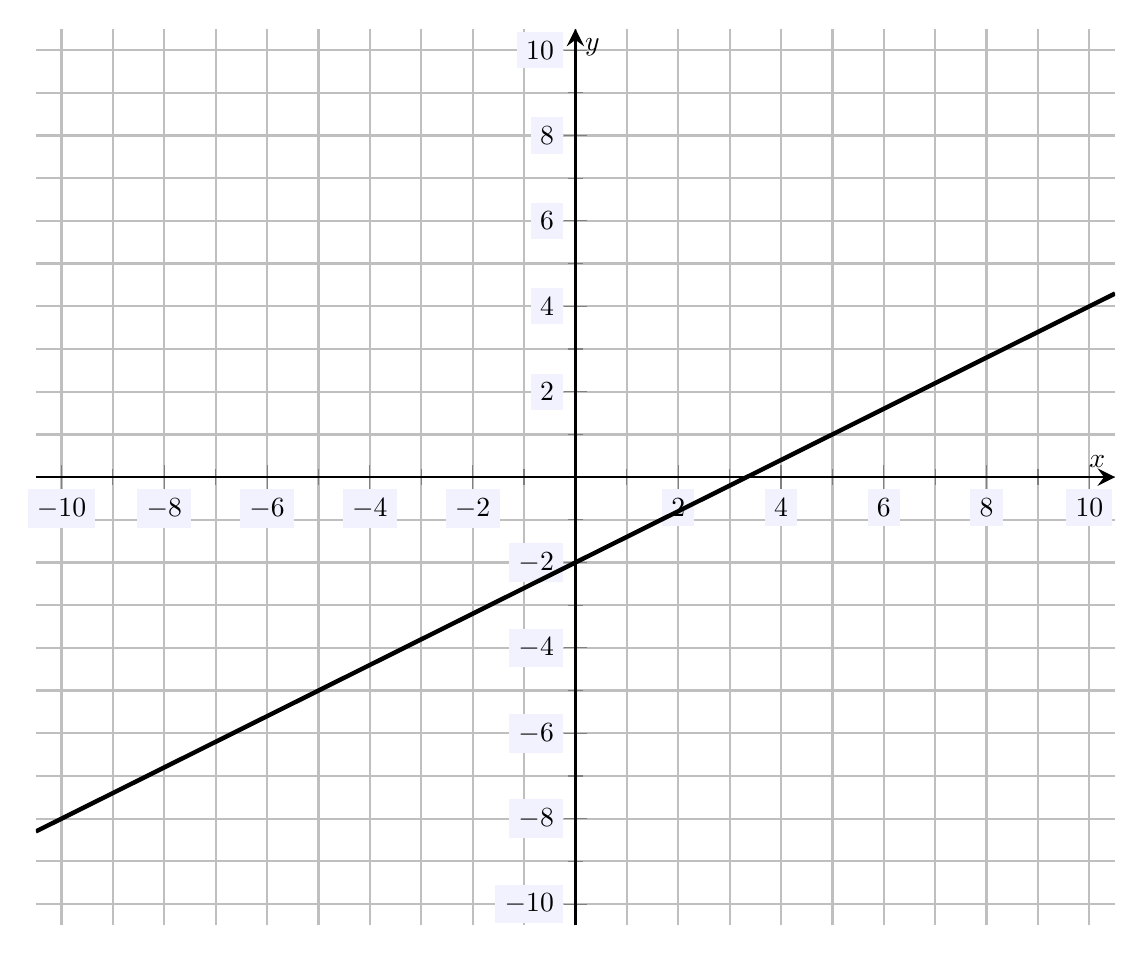
\begin{tikzpicture}[scale=2,every node/.style={scale=0.5}]
	\begin{axis}[
	grid=both,
	axis lines=middle,
	ticklabel style={fill=blue!5!white},
	xmin= -10.5, xmax=10.5,
	ymin= -10.5, ymax=10.5,
	xtick={-10,-8,-6,-4,-2,0,2,4,6,8,10},
	ytick={-10,-8,-6,-4,-2,0,2,4,6,8,10},
	minor tick = {-10,-9,...,10},
	xlabel=\(x\),ylabel=\(y\),
	]
	\addplot[thick, domain= -10.5:10.5] ({x},{3/5*x - 2});	
	\end{axis}
	\end{tikzpicture}
	}
	\] \pspace

{\itshape Solving for $y$, we have\dots
	\[
	\begin{aligned}
	3x &- 5y= 10 \\[0.3cm]
	-5y&= -3x + 10 \\[0.3cm]
	y&= \dfrac{3}{5}\,x - 2
	\end{aligned}
	\] \pspace
We can then easily find two points on the line to connect with a straight line, as in the plot above: \pspace
	\[
	\begin{aligned}
	y(5)&= \dfrac{3}{5} \cdot 5 - 2= 3 - 2= 1 \squiggle (5, 1) \\[0.3cm]
	y(-5)&= \dfrac{3}{5} \cdot -5 - 2= -3 - 2= -5 \squiggle (-5, -5)
	\end{aligned}
	\]
}



\newpage



% Question 4
\newpage
\question[6] Two lines are given below. Determine whether these lines are the same or parallel. Determine also whether these lines intersect or not. If so, determine whether they intersect perpendicularly. 
	\[
	\begin{aligned}
	\ell_1&: & y&= 8 - \dfrac{5}{6}\,x \\
	\ell_2&: & 6x &+ 5y= 15
	\end{aligned}
	\] \pspace

{\itshape Solving for $y$ in the second line, we have\dots \pspace
	\[
	\begin{aligned}
	6x &+ 5y= 15 \\[0.3cm]
	5y&= -6x + 15 \\[0.3cm]
	y&= -\dfrac{6}{5}\,x + 3
	\end{aligned}
	\] \pspace
Therefore, the lines are\dots \pspace
	\[
	\begin{aligned}
	\ell_1&: & y&= 8 - \dfrac{5}{6}\,x \\
	\ell_2&: & y&= -\dfrac{6}{5}\,x + 3
	\end{aligned}
	\]  \pspace
The slope of the first line is $m_1= -\frac{5}{6}$ and the slope of the second line is $m_2= -\frac{6}{5}$. Because $m_1 \neq m_2$, the lines cannot be the same or parallel. Therefore, the lines must intersect. However, the negative reciprocal of $m_1= -\frac{5}{6}$ is $\frac{6}{5} \neq m_2$. Therefore, the lines do not intersect perpendicularly. 
}



\newpage



% Question 5
\newpage
\question[6] A table of values for a linear function $f(x)$ is given below.
	\begin{table}[!ht]
	\centering
	\begin{tabular}{r||rrrrrrrrrrr}
	$x$ & $-12$ & $-8$ & $-4$ & $\phantom{-}4$ & $\phantom{-}8$ & $\phantom{-}12$ \\ \hline
	$f(x)$ & $21$ & $18$ & $15$ & $9$ & $6$ & $3$
	\end{tabular}
	\end{table} \par
Determine the equation for $f(x)$. \pspace

{\itshape Clearly, the line is not vertical so that we know $f(x)= mx + b$. First, we compute the slope of $f(x)$ using the points $(4, 9)$ and $(8, 6)$ (although any two distinct points would suffice):
	\[
	m= \dfrac{9 - 6}{4 - 8}= \dfrac{3}{-4}= -\dfrac{3}{4}
	\]
Then $f(x)= -\frac{3}{4}x + b$. Because $(4, 9)$ is on the line, it satisfies the equation for the line:
	\[
	\begin{aligned}
	f(x)&= -\dfrac{3}{4}\,x + b \\[0.3cm]
	f(4)&= -\dfrac{3}{4} \cdot 4 + b \\[0.3cm]
	9&= -3 + b \\[0.3cm]
	12&= b
	\end{aligned}
	\]
Therefore, $f(x)= -\frac{3}{4}\,x + 12$. 
}



\newpage



% Question 6
\newpage
\question[6] Find the equation of the line that contains the points $(-10, 15)$ and $(2, -1)$. \pspace

{\itshape Clearly, the line is not vertical so that we know $y= mx + b$. First, we compute the slope of the line: \pspace 
	\[
	m= \dfrac{15 - (-1)}{-10 - 2}= \dfrac{16}{-12}= -\dfrac{4}{3}
	\] \pspace
Then $y= -\frac{4}{3}x + b$. Because $(2, -1)$ is on the line, it satisfies the equation for the line: \pspace
	\[
	\begin{aligned}
	y&= -\dfrac{4}{3}\,x + b \\[0.3cm]
	-1&= -\dfrac{4}{3} \cdot 2 + b \\[0.3cm]
	-1&= -\dfrac{8}{3} + b \\[0.3cm]
	b&= -1 + \dfrac{8}{3} \\[0.3cm]
	b&= \dfrac{-3}{3} + \dfrac{8}{3} \\[0.3cm]
	b&= \dfrac{5}{3}
	\end{aligned}
	\] \pspace
Therefore, $f(x)= -\frac{4}{3}\,x + \frac{5}{3}= \frac{5 - 4x}{3}$.
}



\newpage



% Question 7
\newpage
\question[6] Determine the equation of the line that contains the point $(6, 10)$ and is perpendicular to the line $y= -1$. \pspace 

{\itshape Because the line $y= -1$ is horizontal, a line perpendicular to this line must be vertical, i.e. of the form $x= M$ for some $M$. Because the line passes through the point $(6, 10)$, it must be that $x= 6$.}



\newpage



% Question 8
\newpage
\question[6] Find the equation of the line that is perpendicular to the line $y= 4 - 5x$ and passes through the $y$-intercept of the line $y= 2x + 3$. \pspace

{\itshape Because the line is perpendicular to $y= 4 - 5x$ (which is not horizontal), the line is not vertical. Therefore, the line has the form $y= mx + b$. Because this line is perpendicular to $y= 4 - 5x$, which has slope $-5$, the slope of the line must be $m= -(\frac{1}{-5})= \frac{1}{5}$. Then we know that $y= \frac{1}{5}\,x + b$. \pspace

Now because $y(0)= 2(0) + 3= 0 + 3= 3$, the $y$-intercept of $y= 2x + 3$ is the point $(0, 3)$. Because this point lies along the line $y= \frac{1}{5}\,x + b$, we know that it satisfies the equation of the line, i.e.
	\[
	\begin{aligned}
	y&= \dfrac{1}{5}\,x + b \\[0.3cm]
	3&= \dfrac{1}{5} \cdot 0 + b \\[0.3cm]
	3&= b
	\end{aligned}
	\]
Therefore, $y= \frac{1}{5}\,x + 3= \frac{x + 15}{5}$. 
}



\newpage



% Question 9
\newpage
\question[6] A researcher creates a model to predict adolescent male's weight (in lbs) from their height (in cm). The model is $W(h)= 2.6h - 17.3$.
	\begin{enumerate}[(a)]
	\item Is the model linear? Explain.
	\item Determine the slope of $W(h)$. Interpret the slope in context.
	\item Determine the $y$-intercept of $W(h)$. Does the $y$-intercept have meaning in this context? Explain.
	\end{enumerate} \pspace

{\itshape
\begin{enumerate}[(a)]
\item The model $W(h)= 2.6h - 17.3$ has the form $y= mx + b$, where $x= t$, $m= 2.6$, and $b= -17.3$. Therefore, $W(h)$ is linear. \pspace

\item From (a), we know that the slope is $m= 2.6$. Interpreting $m= 2.6= \frac{2.6}{1}$ as $\frac{\Delta y}{\Delta x}$ and using the fact that $x$ has units of cm and $y$ has units of lbs, we see that the slope represents that the model says that for each addition centimeter of height, an adolescent male should weigh 2.6~lbs more. \pspace

\item Because $W(0)= 2.6(0) - 17.3= -17.3$, the $y$-intercept is $(0, -17.3)$. However, $h= 0$ would represent a male adolescent with heigh 0~cm---which is impossible. Moreover, $W(0)= -17.3$~lb would imply that an adolescent male with height 0~cm would weigh $-17.3$~lb---equally nonsensical. Therefore, the $y$-intercept likely does not have meaning in this context. 
\end{enumerate}
}



\newpage



% Question 10
\newpage
\question[4] Sketch the function $f(x)= 8 - (x + 3)^2$ on the plot below. 
	\[
	\fbox{
	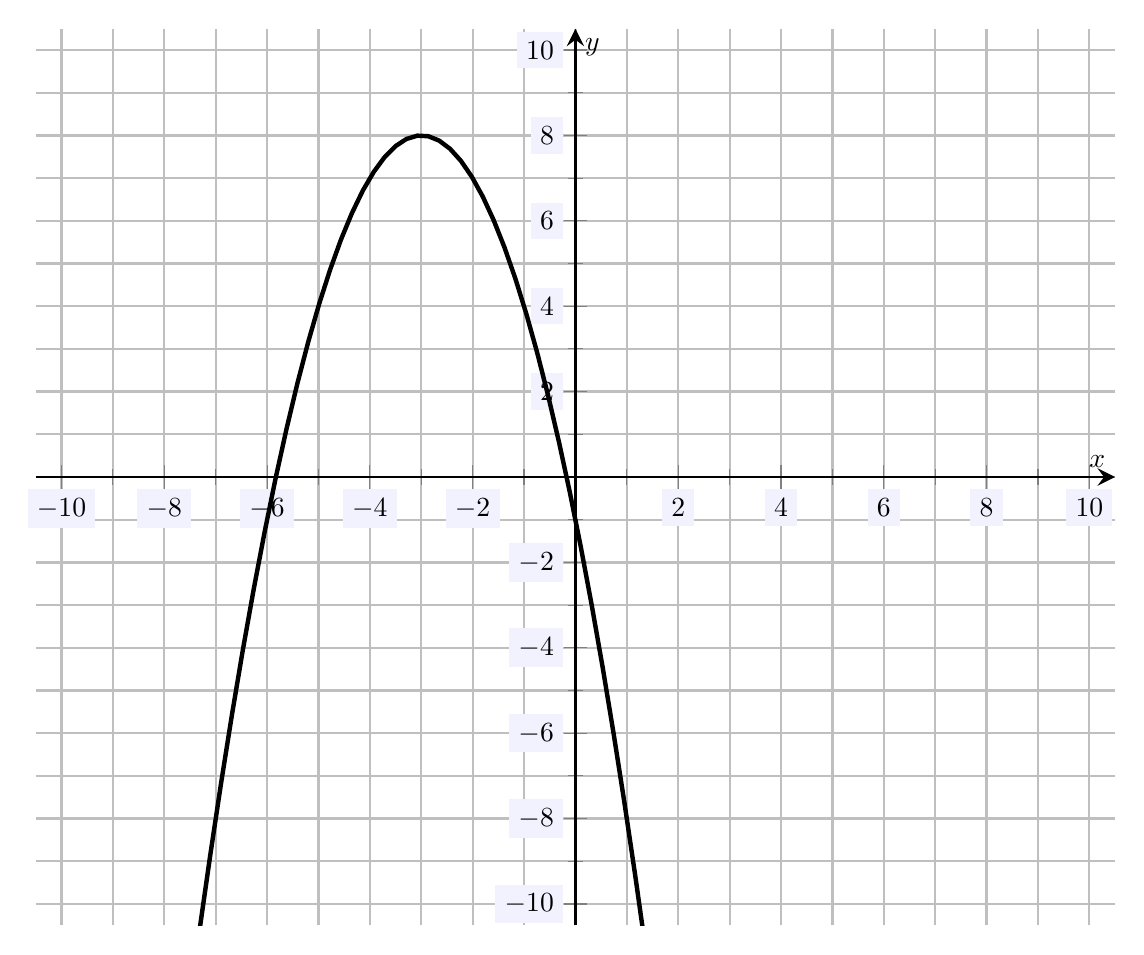
\begin{tikzpicture}[scale=2,every node/.style={scale=0.5}]
	\begin{axis}[
	grid=both,
	axis lines=middle,
	ticklabel style={fill=blue!5!white},
	xmin= -10.5, xmax=10.5,
	ymin= -10.5, ymax=10.5,
	xtick={-10,-8,-6,-4,-2,0,2,4,6,8,10},
	ytick={-10,-8,-6,-4,-2,0,2,4,6,8,10},
	minor tick = {-10,-9,...,10},
	xlabel=\(x\),ylabel=\(y\),
	]
	\addplot[thick, domain= -10.5:10.5, samples=100] ({x},{8 - (x + 3)^2});	
	\end{axis}
	\end{tikzpicture}
	}
	\] \pspace

{\itshape Because $f(x)= 8 - (x + 3)^2$ is in vertex form, we see that the vertex is $(-3, 8)$. Furthermore, because $a= -1 < 0$, we know that the parabola opens downwards. This gives the sketch above.}



\newpage



% Question 11
\newpage
\question[6] Showing all your work, find the vertex form of $y= 2x^2 - 12x + 23$. \pspace

{\itshape 

We complete the square. First, we factor out the 2 to obtain $y= 2(x^2 - 6x + \frac{23}{2})$. Now observe that $\frac{-6}{2}= -3$ and $(-3)^2= 9$. But then\dots \pspace
	\[
	\begin{aligned}
	y&= 2x^2 - 12x + 23 \\[0.3cm]
	y&= 2 \left( x^2 - 6x + \dfrac{23}{2} \right) \\[0.3cm]
	y&= 2 \left( x^2 - 6x + (9 - 9) + \dfrac{23}{2} \right) \\[0.3cm]
	y&= 2 \left( (x^2 - 6x + 9) - 9 + \dfrac{23}{2} \right) \\[0.3cm]
	y&= 2 \left( (x^2 - 6x + 9) - \dfrac{18}{2} + \dfrac{23}{2} \right) \\[0.3cm]
	y&= 2 \left( (x - 3)^2 + \dfrac{5}{2} \right) \\[0.3cm]
	y&= 2(x - 3)^2 + 5
	\end{aligned}
	\]
}



\newpage



% Question 12
\newpage
\question[6] Showing all your work, factor the polynomial $x^2 - 22x - 48$. \pspace

{\itshape
	\begin{table}[!ht]
	\centering
	\underline{\bfseries 48} \pvspace{0.2cm}
	\begin{tabular}{rr}
	$1 \cdot -48$ & $-47$ \\
	$-1 \cdot 48$ & $47$ \\ \hline
	\multicolumn{1}{|r}{$2 \cdot -24$} & \multicolumn{1}{r|}{$-22$} \\ \hline
	$-2 \cdot 24$ & $22$ \\
	$3 \cdot -16$ & $-13$ \\
	$-3 \cdot 16$ & $13$ \\
	$4 \cdot -12$ & $-8$ \\
	$-4 \cdot 12$ & $8$ \\
	$6 \cdot -8$ & $-2$ \\
	$-6 \cdot 8$ & $2$ \\
	\end{tabular}
	\end{table}

Therefore,
	\[
	x^2 - 22x - 48= (x + 2)(x - 24)
	\]
}



\newpage



% Question 13
\newpage
\question[6] Showing all your work, factor the polynomial $5x^2 + 19x - 4$. \pspace

	\begin{table}[!ht]
	\centering
	\underline{\bfseries 4} \pvspace{0.1cm}
	\begin{tabular}{c}
	$1 \cdot -4$ \\
	$-1 \cdot 4$ \\
	$2 \cdot -2$
	\end{tabular}
	\end{table} 

Then as $5= 1 \cdot 5$, we have\dots \pspace
	\[
	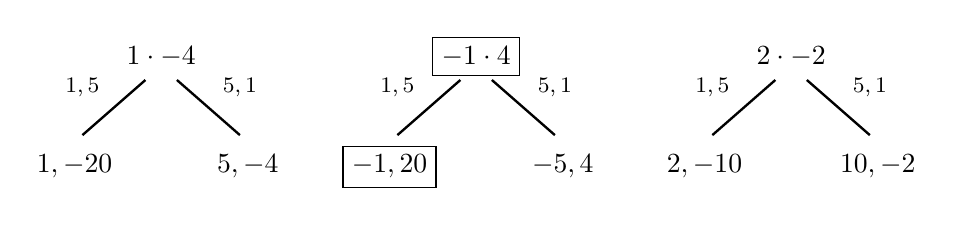
\begin{tikzpicture}
	\node at (0,0) {$1 \cdot -4$};
	\node at (-1.0,-0.4) {\footnotesize$1, 5$};
	\draw[line width=0.03cm,label={1}] (-0.2,-0.3) -- (-1,-1);
	\node at (-1.1,-1.4) {$1, -20$};
	\node at (1.0,-0.4) {\footnotesize$5, 1$};
	\draw[line width=0.03cm] (0.2,-0.3) -- (1,-1);
	\node at (1.1,-1.4) {$5, -4$};	
	
	\tikzset{shift={(4,0)}}

	\node at (0,0) {\framebox{$-1 \cdot 4$}};
	\node at (-1.0,-0.4) {\footnotesize$1, 5$};
	\draw[line width=0.03cm,label={1}] (-0.2,-0.3) -- (-1,-1);
	\node at (-1.1,-1.4) {\framebox{$-1, 20$}};
	\node at (1.0,-0.4) {\footnotesize$5, 1$};
	\draw[line width=0.03cm] (0.2,-0.3) -- (1,-1);
	\node at (1.1,-1.4) {$-5, 4$};

	\tikzset{shift={(4,0)}}

	\node at (0,0) {$2 \cdot -2$};
	\node at (-1.0,-0.4) {\footnotesize$1, 5$};
	\draw[line width=0.03cm,label={1}] (-0.2,-0.3) -- (-1,-1);
	\node at (-1.1,-1.4) {$2, -10$};
	\node at (1.0,-0.4) {\footnotesize$5, 1$};
	\draw[line width=0.03cm] (0.2,-0.3) -- (1,-1);
	\node at (1.1,-1.4) {$10, -2$};
	\end{tikzpicture}
	\] \pspace

Therefore, 
	\[
	5x^2 + 19x - 4= (5x - 1)(x + 4)
	\]



\newpage



% Question 14
\newpage
\question[6] Showing all your work, solve the equation $2x= 24 - x^2$. \pspace

{\itshape
	\[
	\begin{aligned}
	2x= 24 &- x^2 \\[0.3cm]
	x^2 + 2x - 24&= 0 \\[0.3cm]
	(x + 6)(x - 4)&= 0
	\end{aligned}
	\] \pspace
Then either $x + 6= 0$, which implies $x= -6$, or $x - 4= 0$, which implies that $x= 4$. Therefore, we have\dots \pvspace{0.1cm}
	\[
	x= -6,\, 4
	\]
}



\newpage



% Question 15
\newpage
\question[6] Showing all your work, use the quadratic equation to solve $2x^2= 4x - 10$. \pspace

{\itshape First, we rewrite the equation:
	\[
	\begin{aligned}
	2x^2= 4x &- 10 \\[0.3cm]
	2x^2 - 4x + 10&= 0
	\end{aligned}
	\] 
Then we have\dots \pspace
	\[
	\begin{aligned}
	x&= \dfrac{-b \pm \sqrt{b^2 - 4ac}}{2a} \\[0.3cm]
	x&= \dfrac{-(-4) \pm \sqrt{(-4)^2 - 4(2)(10)}}{2(2)} \\[0.3cm]
	x&= \dfrac{4 \pm \sqrt{16 - 80}}{4} \\[0.3cm]
	x&= \dfrac{4 \pm \sqrt{-64}}{4} \\[0.3cm] 
	x&= \dfrac{4 \pm \sqrt{-64}}{4} \\[0.3cm] 
	x&= \dfrac{4 \pm \sqrt{64}i}{4} \\[0.3cm] 
	x&= \dfrac{4 \pm 8i}{4} \\[0.3cm] 
	x&= 1 \pm 2i 
	\end{aligned}
	\] \pspace
Then either $x= 1 + 2i$ or $x= 1 - 2i$. Therefore, $x= 1 - 2i, 1 + 2i$. 
}



\newpage



% Question 16
\newpage
\question[4] Consider the quadratic function $f(x)= x^2 - 6x + 4$. Use the discriminant of $f(x)$ to show that $f(x)$ does not factor `nicely', then use the quadratic formula to factor $f(x)$. \pspace

{\itshape We know that $D= b^2 - 4ac$. For $f(x)$, we have $a= 1$, $b= -6$, and $c= 4$. But then \pspace
	\[
	D= b^2 - 4ac= (-6)^2 - 4(1)4= 36 - 16= 20= 2^2 \cdot 5
	\] \pspace
Because 20 is not a perfect square, the polynomial $f(x)= x^2 - 6x + 4$ does not factor `nicely.' To find a factorization of $f(x)$, we find the roots of $f(x)$: \pspace
	\[
	\begin{aligned}
	x&= \dfrac{-b \pm \sqrt{b^2 - 4ac}}{2a} \\[0.3cm]
	x&= \dfrac{-(-6) \pm \sqrt{(-6)^2 - 4(1)(4)}}{2(1)} \\[0.3cm]
	x&= \dfrac{6 \pm \sqrt{36 - 16}}{2} \\[0.3cm]
	x&= \dfrac{6 \pm \sqrt{20}}{2} \\[0.3cm] 
	x&= \dfrac{6 \pm \sqrt{4 \cdot 5}}{2} \\[0.3cm] 
	x&= \dfrac{6 \pm 2\sqrt{5}}{2} \\[0.3cm] 
	x&= 3 \pm \sqrt{5}
	\end{aligned}
	\] \pspace
Then the roots are $r_1= 3 + \sqrt{5}$ and $r_2= 3 - \sqrt{5}$. Then we have\dots 
	\[
	f(x)= x^2 - 6x + 4= a(x - r_1)(x - r_2)= 1 \big(x - (3 + \sqrt{5}) \big) \big(x - (3 - \sqrt{5}) \big)= \big(x - (3 + \sqrt{5}) \big) \big(x - (3 - \sqrt{5}) \big)
	\]
}



\newpage



% Question 17
\newpage
\question[10] Consider the function $f(x)= 3x^2 - 15x + 20$. 
	\begin{enumerate}[(a)]
	\item Determine if the parabola is concave up or concave down. 
	\item Determine the axis of symmetry of $f(x)$. 
	\item Determine the vertex of $f(x)$.
	\item Does $f(x)$ have a maximum or minimum value? Explain. 
	\item Find the maximum or minimum value of $f(x)$ from (d).  
	\end{enumerate} \pspace

{ \itshape
\begin{enumerate}[(a)]
\item Because $a= 3 > 0$, the parabola opens upwards, i.e. is concave up (or convex). \pspace

\item We know the $x$-coordinate of the vertex occurs when $x= \frac{-b}{2a}$. But then\dots
	\[
	x= \dfrac{-b}{2a}= \dfrac{-(-15)}{2(3)}= \dfrac{15}{2(3)}= \dfrac{5}{2}
	\]
Therefore, the axis of symmetry is $x= \frac{5}{2}$. \pspace

\item We know the $x$-coordinate of the vertex is $x= \frac{5}{2}$. Then the $y$-value is\dots
	\[
	f\left(\frac{5}{2}\right)= 3\left( \dfrac{5}{2} \right)^2 - 15 \cdot \dfrac{5}{2} + 20= 3 \cdot \dfrac{25}{4} - \dfrac{75}{2} + 20= \dfrac{75}{4} - \dfrac{150}{4} + \dfrac{80}{4}= \dfrac{5}{4}
	\]
Therefore, the vertex is $(\frac{5}{2}, \frac{5}{4})$. \pspace

\item Because $a= 3 > 0$, the parabola opens upwards, i.e. is concave up or convex. But then $f(x)$ has a minimum value. \pspace

\item We know the minimum value for $f(x)$ occurs at the vertex, which from (c) is $(\frac{5}{2}, \frac{5}{4})$. But then the minimum value for $f(x)$ is $\frac{5}{4}$. 
\end{enumerate}
}


\end{questions}
\end{document}